\chapter{System Evaluation}
This chapter presents the evaluation of the system infrastructure, architecture and the verification and validation techniques used. Also results from the machine 
learning models were presented and analyzed. 
system are discussed and summarized in this chapter. 

\section{System Verification}
Several components of the system interact together to perform the functionalities of the system and thus it is important to verify that each component works as 
expected. Each component was tested as a separate unit employing a test-driven development approach. An automated test suites were written for every functional component
of the system to test its correctness and reliability.
\subsection{Unit Testing}
An automated unit testing strategy was employed to verify continuously evolving components of the system. This strategy was also utilized for Regression Testing
to detect any breaking changes that may be introduced by new codes.
Users data were derived from different collections (Biometric data \& Performance data) of the Firestore database and were combined together as a single tuple in the 
relational database.  Testing effort was focused on boiler-plate CRUD (Create, Read, Update, Delete) required to synchronize data between the databases and service 
the various API endpoints. Test cases for Asynchronous Javascript and XML (AJAX) calls were written verify integrity of data being fetched from the API endpoints. 
Unit tests suites were developed using Mocha for both the Dashboard and Controller components. Fig~\ref{image:test_cases} shows the test cases developed for the 
system. 

\begin{figure}[H]
    \centering
    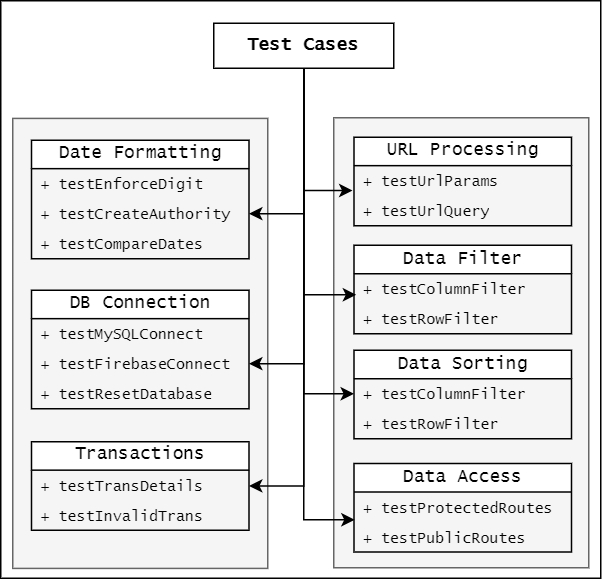
\includegraphics[width=0.8\textwidth]{images/test_cases.png}
    \caption{Test Cases}
    \label{image:test_cases}
\end{figure}

\section{System Validation}

Validating the system involved ensuring that the system meets the stated requirements and objectives. Acceptance testing was carried out to verify that the 
proposed functionalities of the system were implemented satisfactorily. The Acceptance testing was carried out with real data with the help of the supervising
lecturer and volunteers. Functional and non functional testing were carried out to validate the system requirements, performance and security. 
The following metrics were used to validate the system: 
\begin{itemize}
    \item \textbf{Performance} - The system was tested for handling multiple request by simulating multiple users using Postman to send requests. The system satisfactorily
    serviced all requests without any noticeable delay. 
    \item \textbf{Security} - The system was tested for security by attempting to access the API endpoints without the required authentication. Such requests were rejected
    and appropriate error messages and code were returned. 
    \item \textbf{Accessibility} - The system was tested for accessibility using different devices and browsers to ensure a consistent user experience across board and
    validate that AJAX calls were handled correctly across different browser implementations. 
    \item \textbf{Usability} - The system was tested for usability, as the system was designed for non-technical users with the help of volunteers. The User
    Interface were supposed to be minimalistic and provide all functionalities in a single view. The users were able to perform the required tasks without any assistance.
\end{itemize}

\section{Machine Learning Model Evaluation}

\section{Project Objectives}
The initial project objective was to build an enduring infrastructure that can access users data and do real-time analysis. The system was shown to be able to reliably 
perform the stated tasks effectively. The achievement recorded in this project is summarized below:
\begin{itemize}
\item \textbf{Infrastructure} - A cloud-based infrastructure was successfully implemented using Amazon Web Services (AWS) as the cloud provider,  
\end{itemize}



Evaluate your project against the objectives set out in the introduction.
This chapter should present results if applicable and discuss the strengths and weaknesses of your system. This is a clear opportunity for you to 
demonstrate your critical thinking in relation to the project. 